\section{Experimental Evaluation}
\label{sec:experiments}

To validate the proposed mechanism, we utilized an oracle-based experimental methodology. 
We first executed the Malachite protocol using standard round-robin rotation to establish a baseline. 
From the resulting logs, we simulated the score-calculation algorithm to generate an optimized proposer sequence. 
Finally, we re-executed the protocol using this new sequence to measure performance gains. This iterative process was repeated up to six times (\textit{alg-1} through \textit{alg-6}) to observe score stabilization. 

%[???  modificou o proposto antes ????   como o leitor entende ????   gastou tempo do leitor explicando la, agora muda nao sei por que...  ]  
%For these evaluations, we measured \textit{block time} rather than consensus duration, as block time accounts for the full interval from height start to decision, providing a more realistic metric for production environments.

The scoring algorithm used consistent parameters across all tests: uniform node stake, a score range $M=5$, a 50\% consensus threshold ($T=0.5$), $\alpha=3$, $\beta=0.9$, and a 100\% contribution factor ($C=1$). These values were chosen to prioritize rapid convergence in stable network conditions.

We repeated the experimentation with 3 different topologies, respectively cases A, B and C.

\subsubsection{Case A.} 
In the 13-node AWS topology, we evaluated the iterative convergence of the algorithm (\textit{alg}) against the default rotative system (\textit{def}). As shown in \textbf{Fig. \ref{alg2}}, which tracks block times across sequential runs, the high $\alpha$ value allows the scores to stabilize within four iterations. Once stabilized, the algorithm achieves an 8\% performance gain primarily by reducing the frequency of the two most distant nodes in the proposer pool. For comparison, a traditional node-removal strategy (\textit{rem-2}) achieves a slightly higher 10\% gain but incurs a critical cost: 
the two most distant nodes were excluded, reducing the committee size from $N=13$ to $N=11$, which lowers the Byzantine fault tolerance from $F=4$ to $F=3$. Our approach maintains the full committee while achieving comparable performance.

\begin{figure}[htbp]
\centerline{%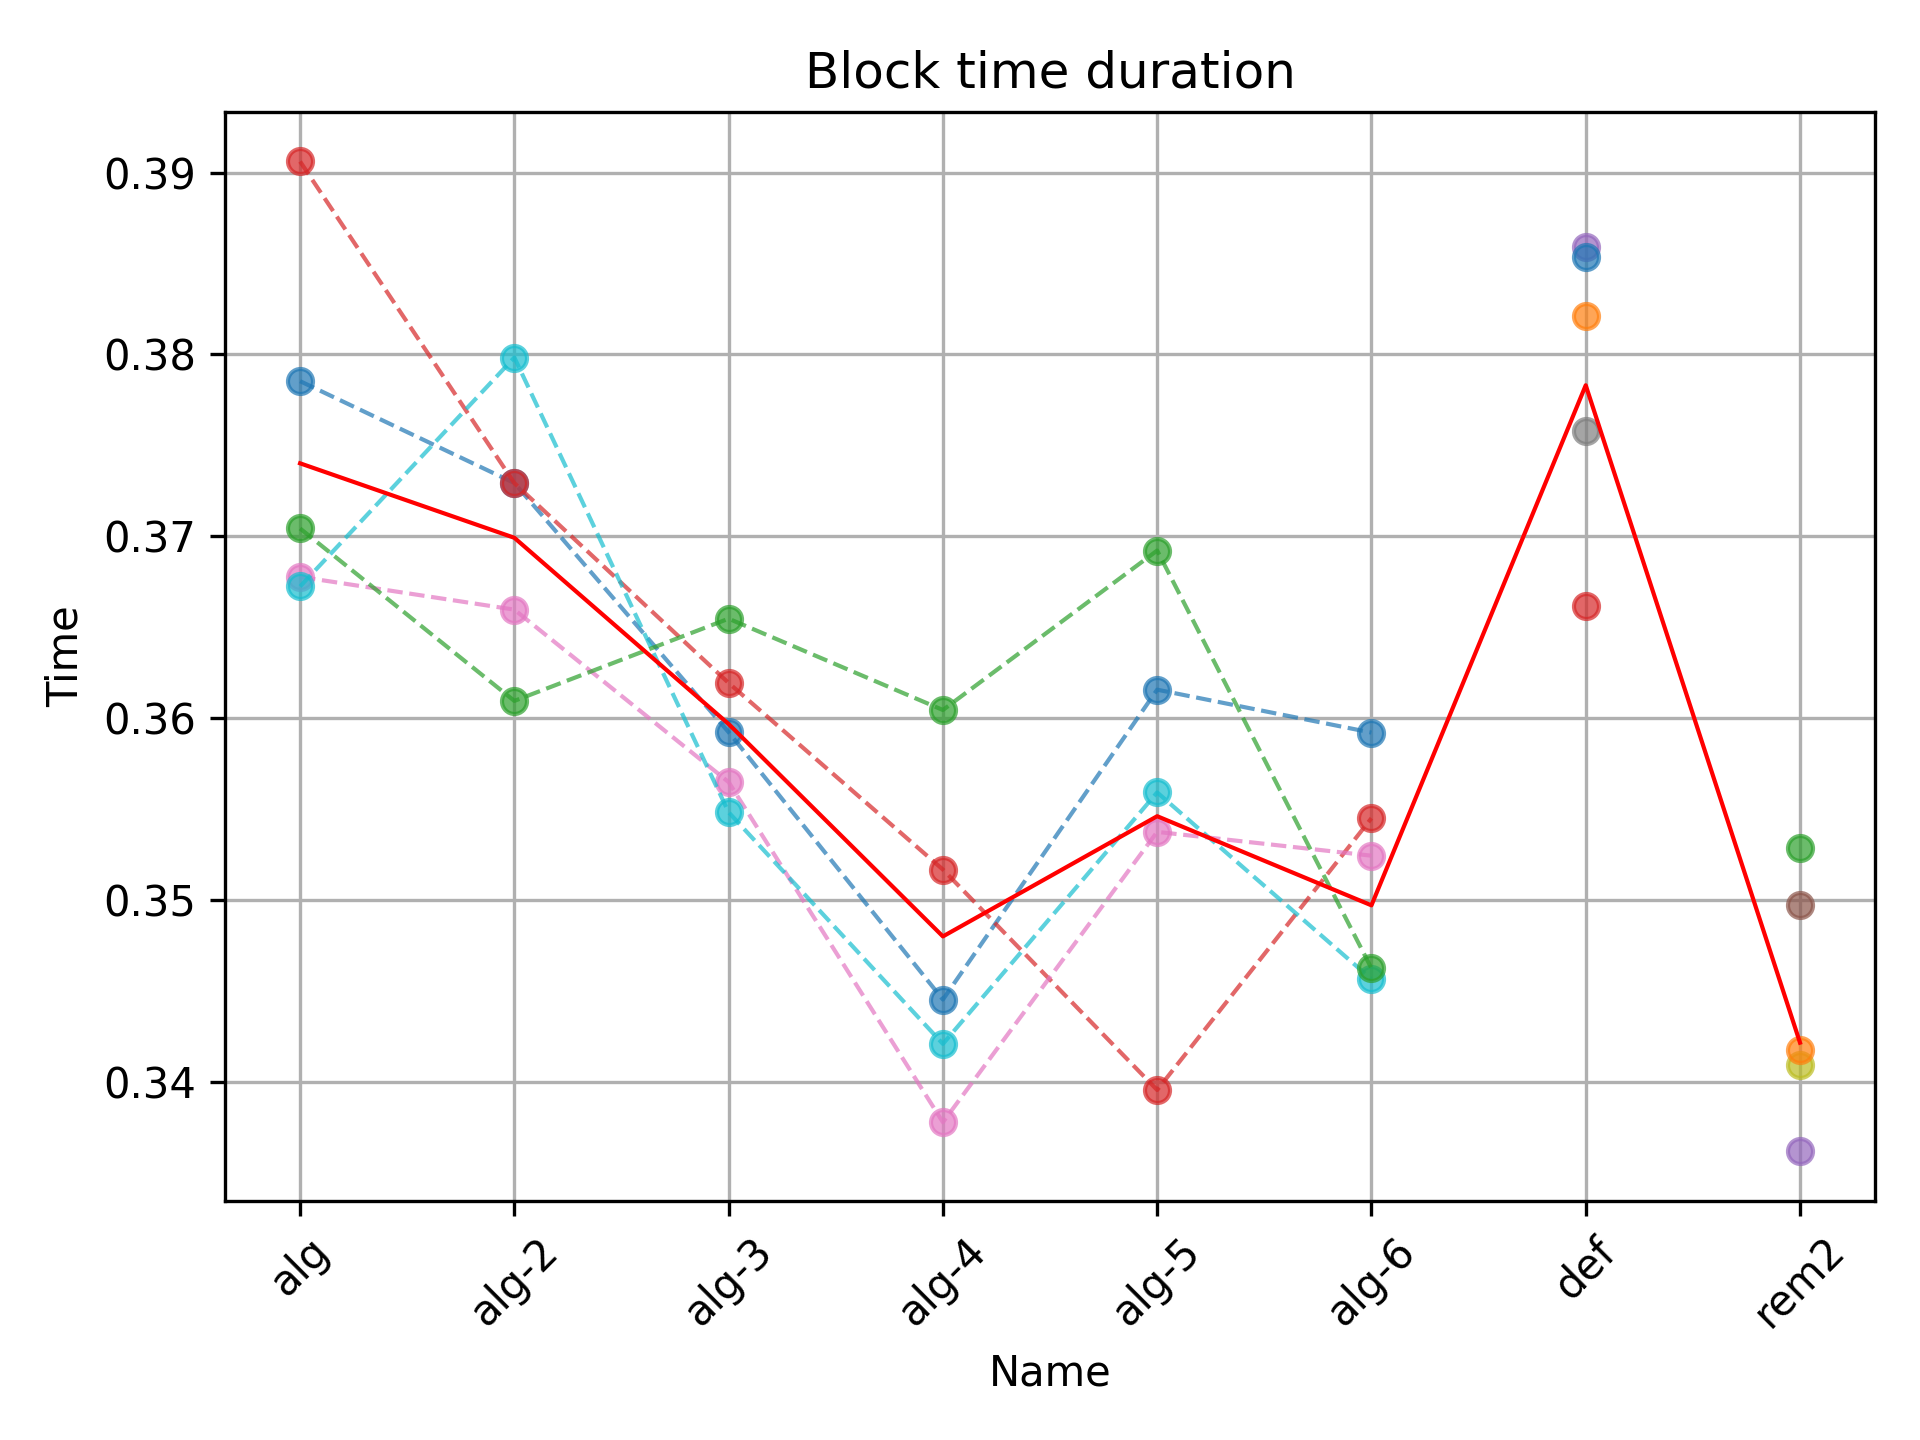
\includegraphics[width=0.5\textwidth]{img/aws13.png}}
 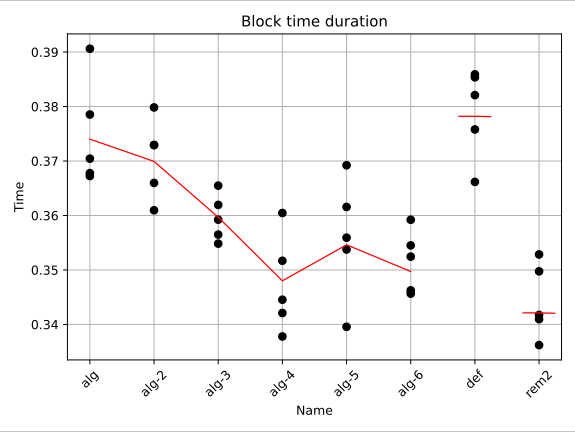
\includegraphics[width=0.6\linewidth]{svgi/awsblock.svg.png}
 %\includesvg[width=\linewidth]{svg/awsblock.svg}
}
%\centerline{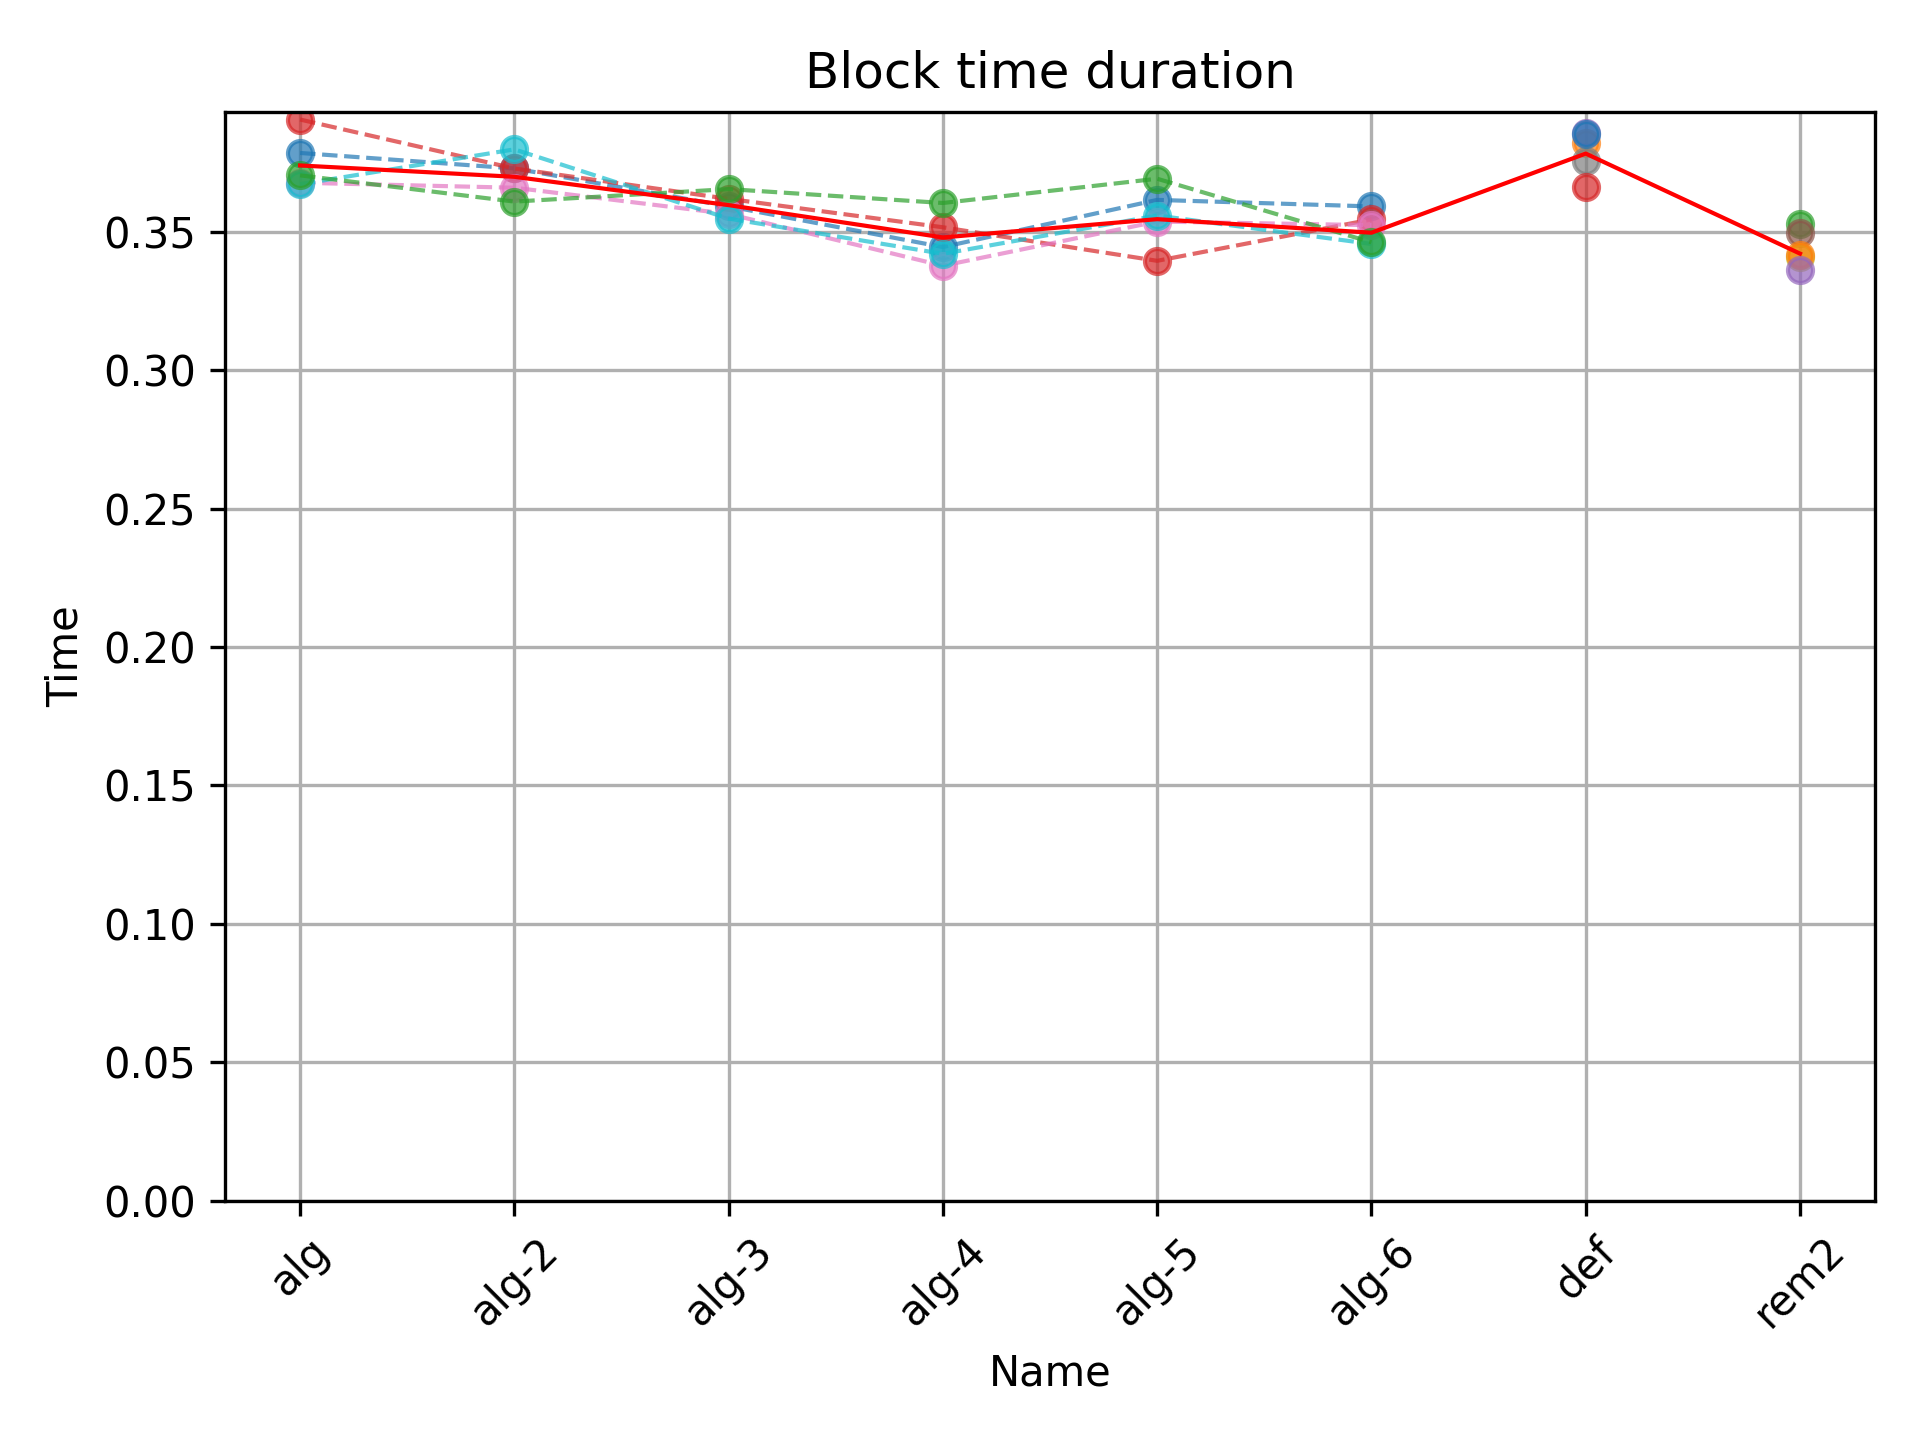
\includegraphics[width=0.3\textwidth]{img/aws13zero.png}}
\caption{Experiment with the topology used for measurements Section 3,
13 AWS zones. 5 runs (each one a plot) per configuration. Red line is the average.}
\label{alg2}
\end{figure}

\subsubsection{Case B.} To assess robustness under variable network conditions, we utilized datasets from \cite{di2025impact} to model two cases, one with 24-hour data and another with 16-month data. In the 14-node 24-hour topology (\textbf{Fig. \ref{alg24}}), the scores stabilized in only three steps, yielding a 30\% improvement on block time at the 80th percentile and a 15\% improvement at the median. This confirms that gains are topology-dependent and also that our mechanism helps filtering out long-tail latencies.

\begin{figure}[htbp]
\centerline{%\includegraphics[width=0.3\textwidth]{img/80percentileBlockDurationAvrg.png}}
 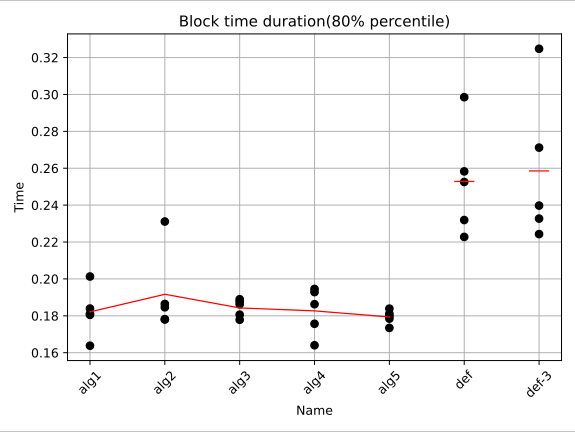
\includegraphics[width=0.6\linewidth]{svgi/dev80th.svg.png}
 %\includesvg[width=\linewidth]{svg/dev80th.svg}
 }
 
%\centerline{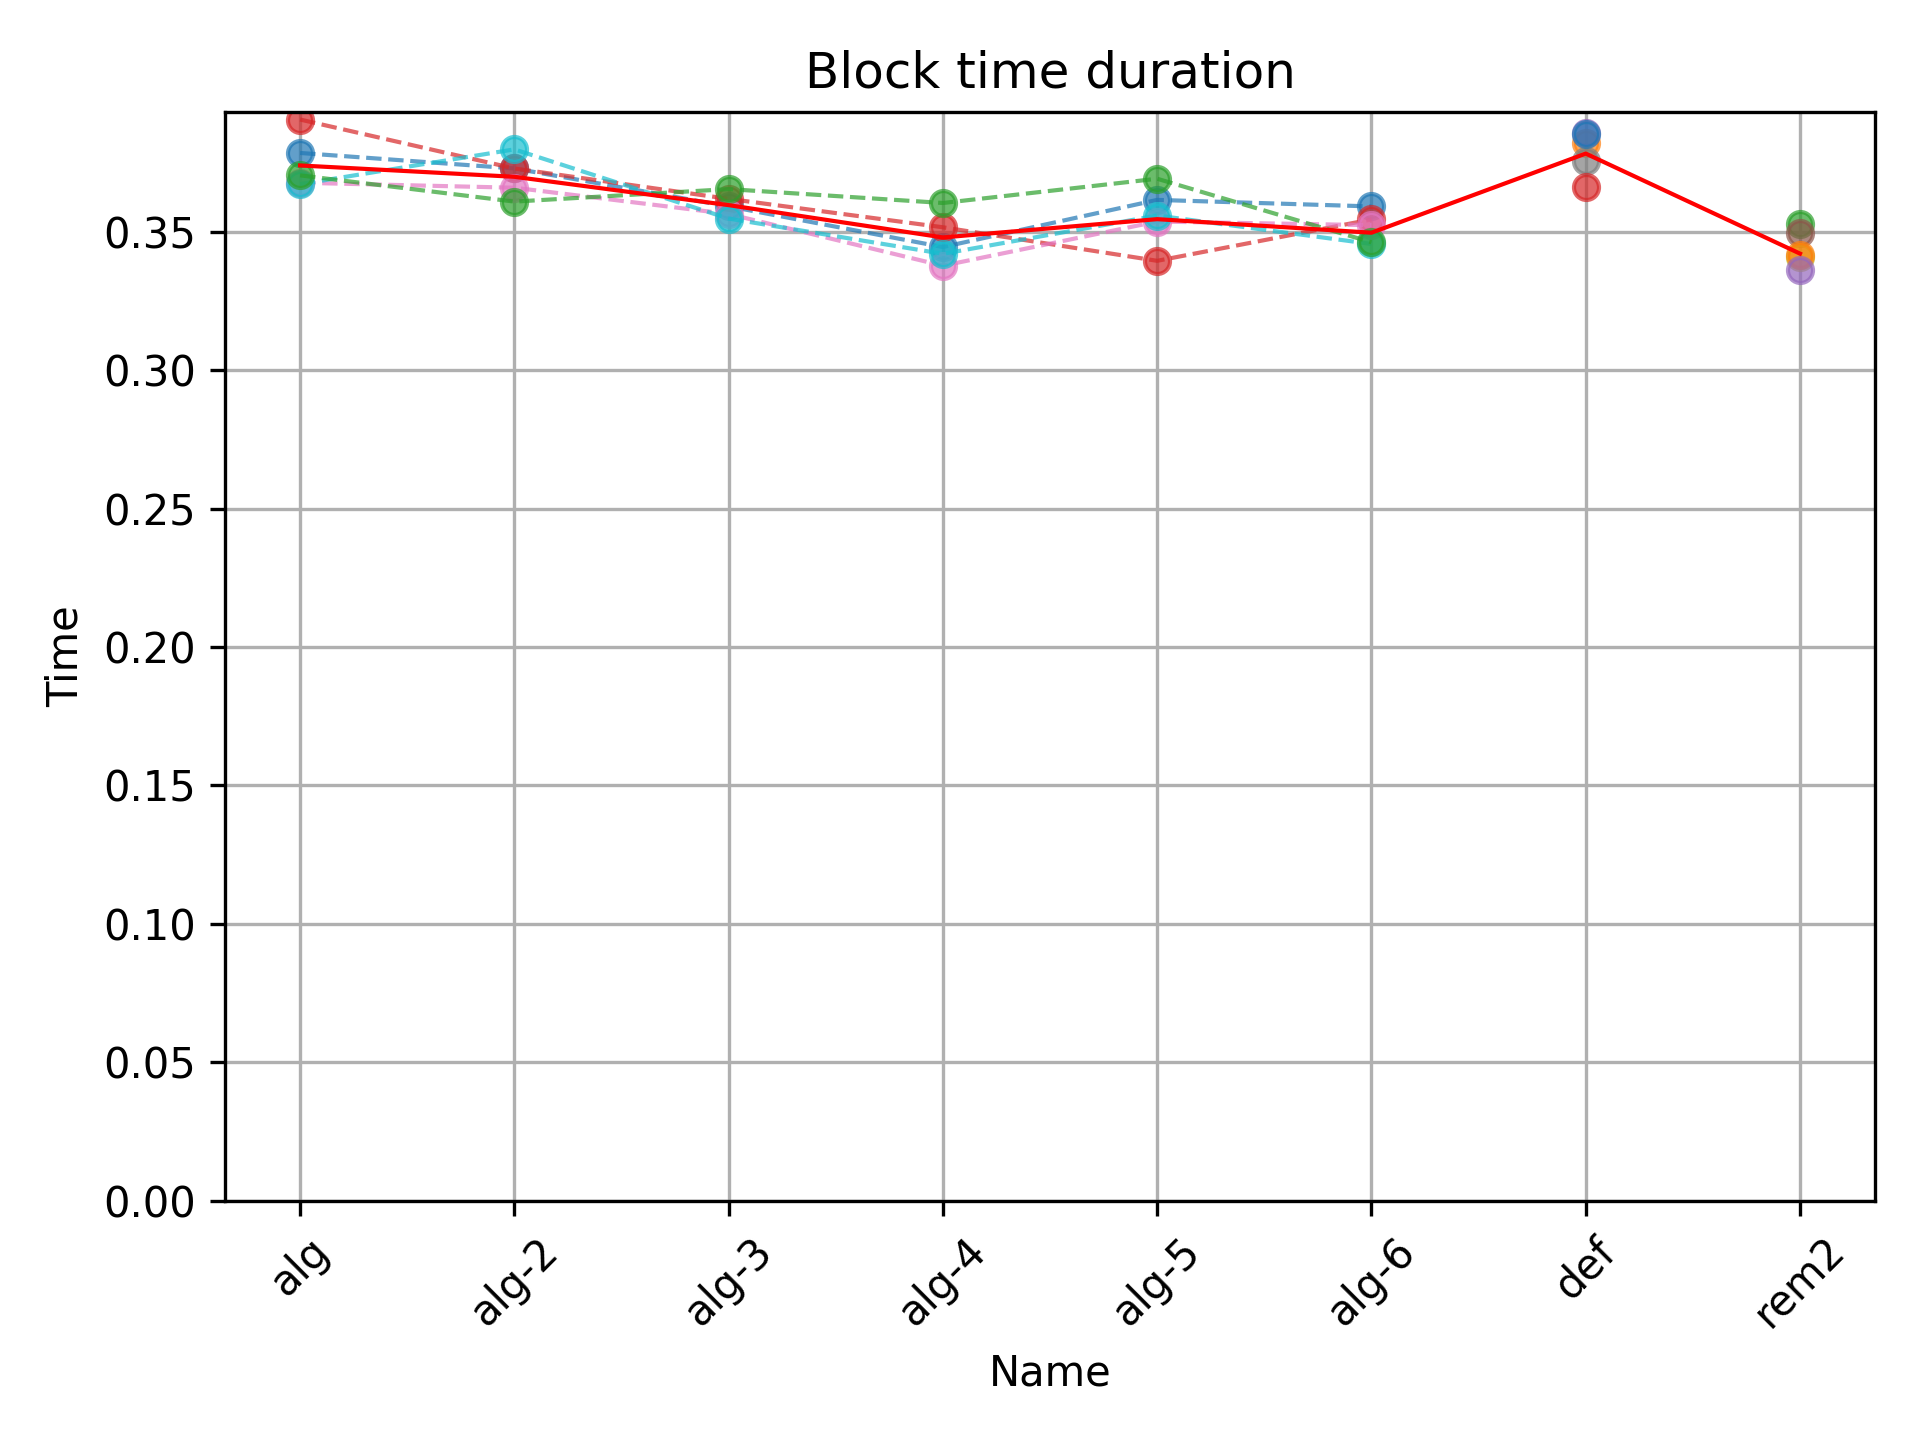
\includegraphics[width=0.3\textwidth]{img/aws13zero.png}}
\caption{Experiment with 24-hour measured 14-node topology from  \cite{di2025impact}.}
\label{alg24}
\end{figure}

\subsubsection{Case C.} Finally, we evaluated a worst-case scenario using a 21-node topology modeled on 16 months of noisy data (\textbf{Fig. \ref{alg3}}). Despite the lack of correlation between latencies of sequential packets, and high latency variability, the algorithm remained robust. It identified subtle patterns to achieve a 6\% gain at the 80th percentile and 3\% at the median without  degrading performance. This stability is crucial for real-world deployment, ensuring that the mechanism provides benefits when patterns exist without introducing overhead during periods of extreme instability.

\begin{figure}[htbp]
\centerline{%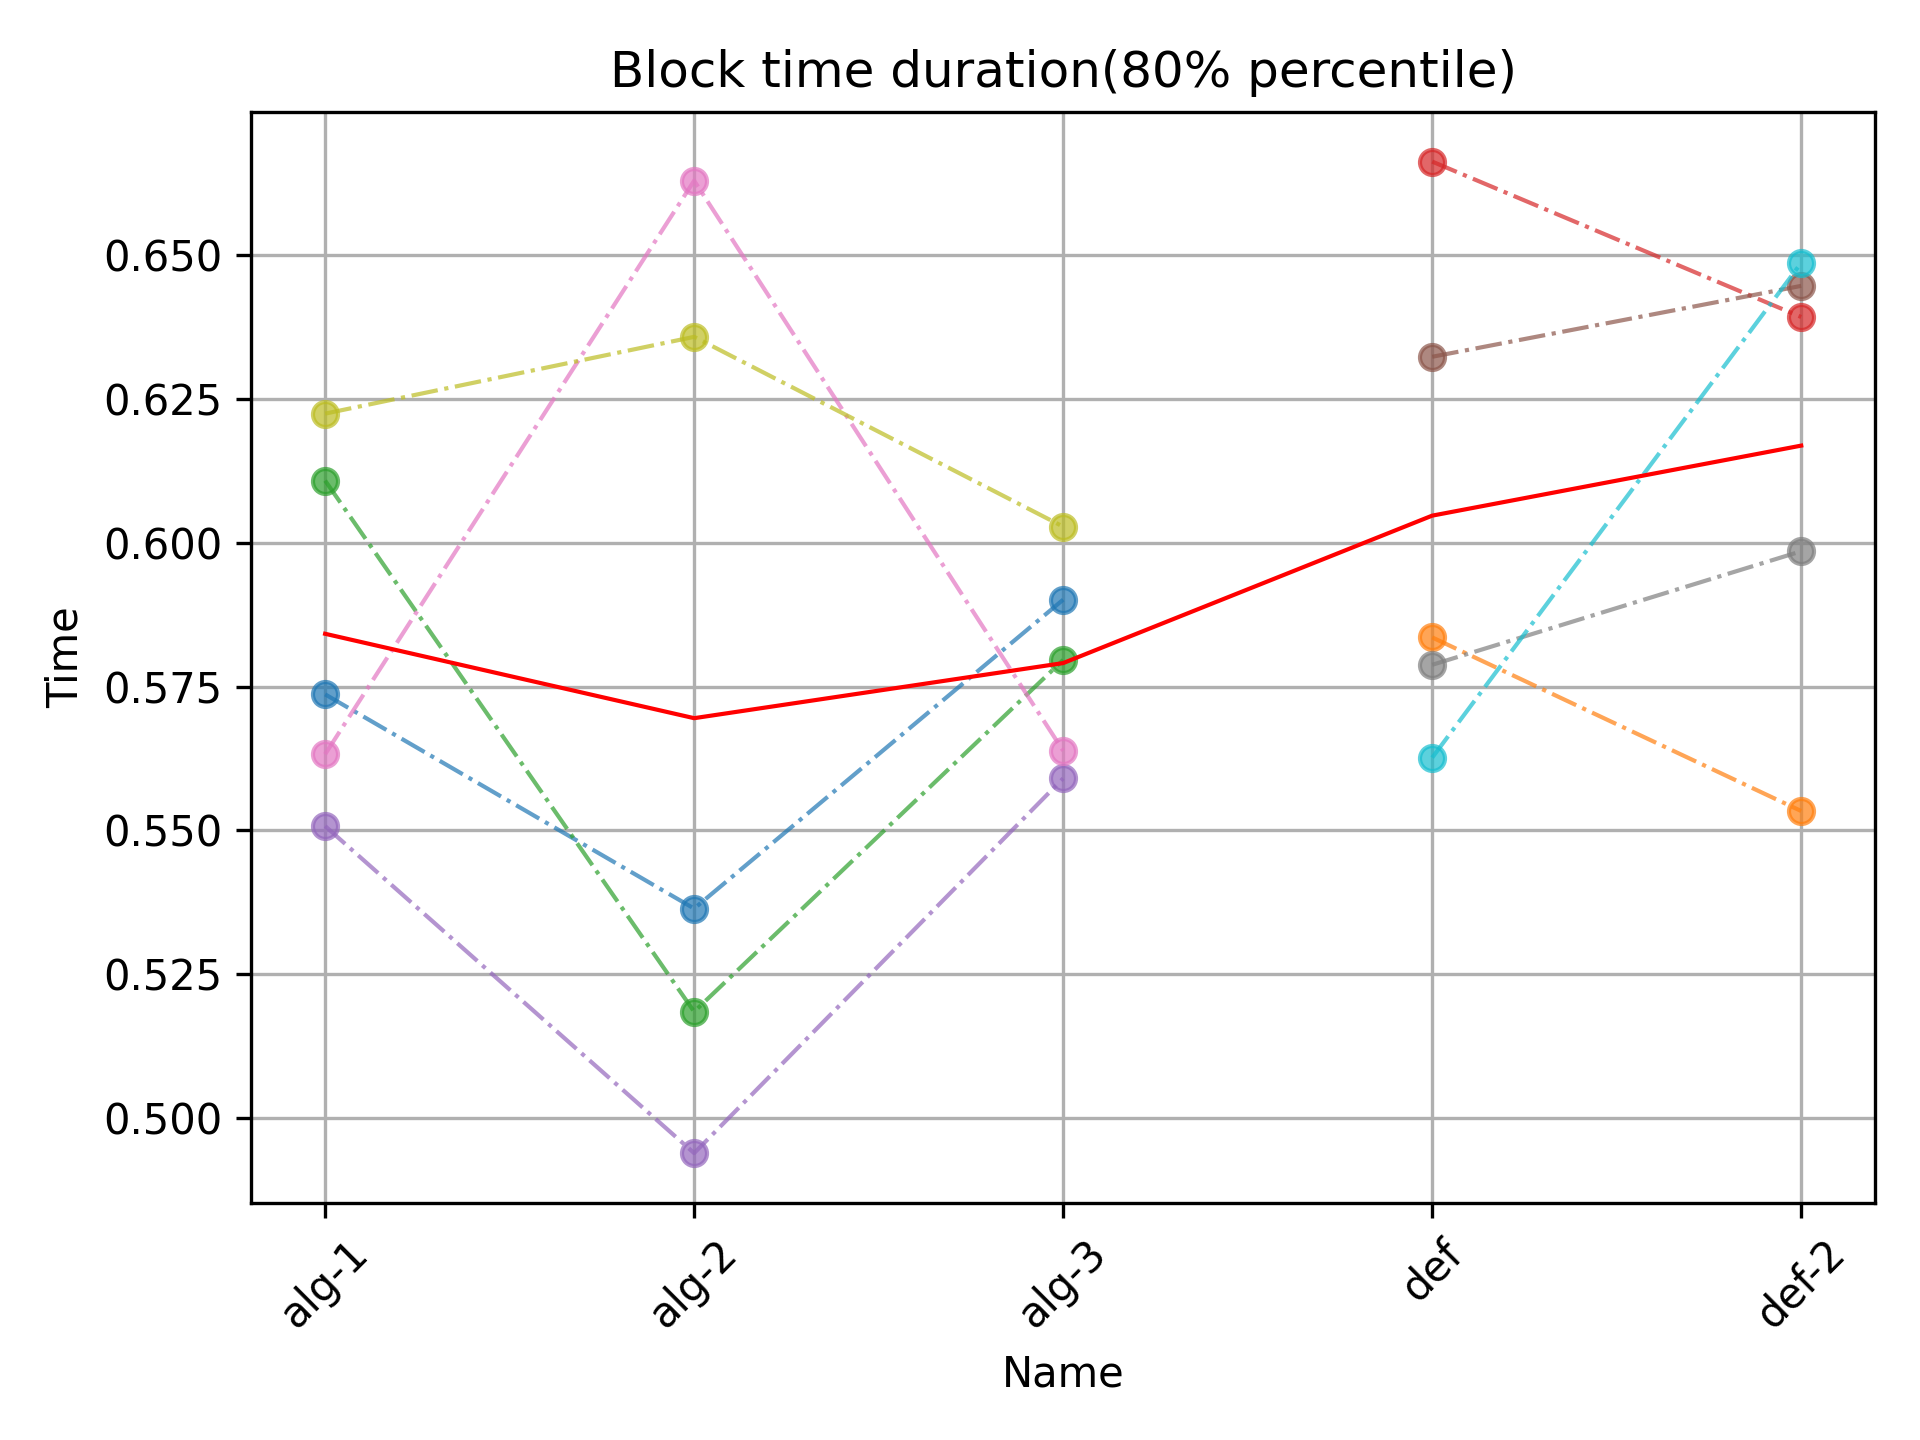
\includegraphics[width=0.3\textwidth]{img/random21.png}}
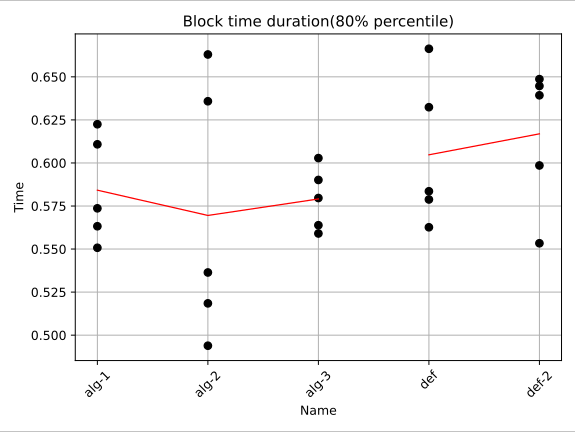
\includegraphics[width=0.6\linewidth]{svgi/rand80th.svg.png}
%\includesvg[width=\linewidth]{svg/rand80th.svg}}
}

%\centerline{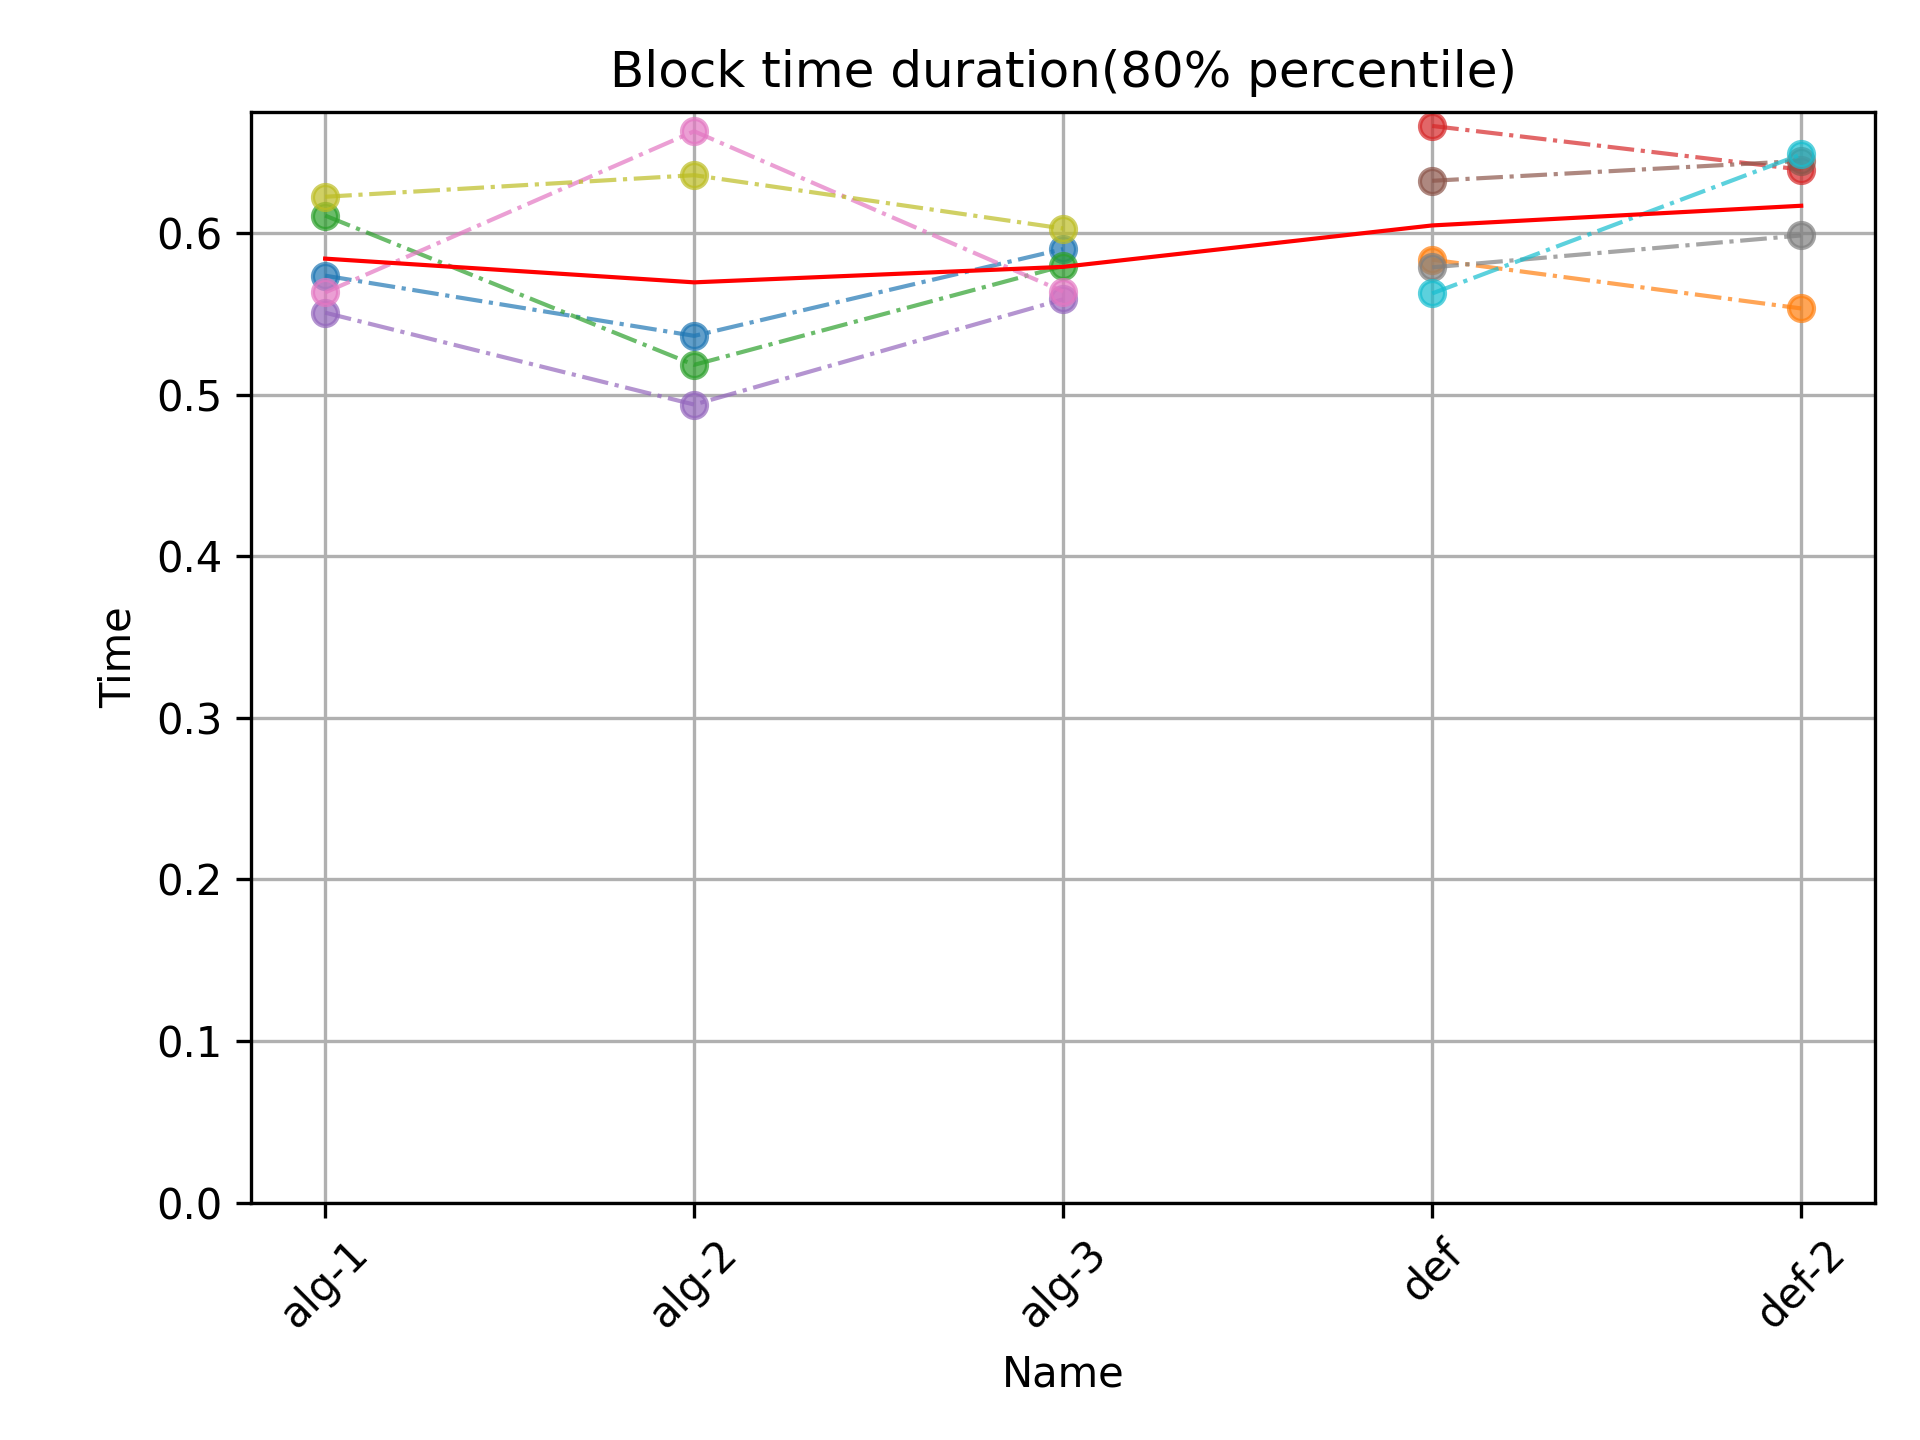
\includegraphics[width=0.3\textwidth]{img/random21zero.png}}
\caption{Experiment with 16 months measures 21 zones topology from \cite{di2025impact}. 5 runs per configuration with 10 rotative runs ????? run run?????}
\label{alg3}
\end{figure}


% \subsection{Multi-instance Evaluation}
% For high-frequency systems where per-instance updates may be excessive, we propose a multi-instance evaluation variant. In this approach, nodes collect local performance observations for $N$ proposals before initiating a distributed consensus on the aggregate results. This modification transforms the score calculation into $S'_n = \beta^N \cdot S_n + \alpha \cdot \sum(L_n)$, where $L_n$ represents a list of $N$ evaluations. This grouping serves two purposes: it significantly reduces the communication overhead and acts as a low-pass filter, smoothing out transient network noise to reveal the underlying performance trends of individual nodes.



% \subsection{Multi-instance Evaluation}

% Noisier topologies or faster systems may not necessitate per-instance update on the score of proposers. In such cases we envision a multi-instance evaluation of proposers, which groups $N$ proposals of a node into a single consensus:

% \begin{enumerate}
%     \item Every time a node $p$ proposes a value, wait for consensus to end and register a local vote.
%     \item Every $N$ times $p$ is the proposer, send the $N$ local votes for the consensus over $p$.
%     \item Reach consensus for each of the $N$ values, defaulting to 0 for impossible consensus (e.g. due to previous nodes leaving the committee).
%     \item After consensus, the network will have a distributed list of values $L_n$ for the node $n$ (e.g. $L_n$ = [-1,-1,0] for $N$=3).
%     \item The network calculates the new value by factoring all $N$ evaluations at once.
% \end{enumerate}

% This turns the previously mentioned $S_n$ calculation into

% $S'_n$ = $\beta^N*Sn + \alpha*sum(L_n)$

% As the vote itself is a simple data structure, for any reasonable choice of $N$ the entire list of votes of a node can fit into a single message. This can further reduce the already small communication cost and also how often consensus happens. A side effect of this is that the larger the $N$ the more is smoothes over any noise in the decisions. This could be useful in networks where nodes exhibit clear performance patterns despite frequent noise.


